\documentclass[12pt]{scrartcl}

\usepackage[T1]{fontenc}
\usepackage[utf8]{inputenc}
\usepackage{amsmath}
\usepackage{amsfonts}
\usepackage{amssymb}
\usepackage{amsbsy}
\usepackage{graphicx}
\usepackage{float}
\usepackage{array}
\usepackage{booktabs}
\usepackage{multirow}
\usepackage{bm}
\usepackage{verbatim}
\usepackage[french]{babel}
\usepackage{color}
\usepackage{url}
\usepackage{fancybox}
\usepackage[stable]{footmisc}
\usepackage[format=plain,labelfont=bf]{caption}
\usepackage{fancyhdr}
\usepackage{natbib}
\usepackage{calc}
\usepackage{textcomp}
\usepackage[pdftex,pdfborder={0 0 0}]{hyperref}
\usepackage{pdfpages}
\usepackage{tikz}
\usetikzlibrary{shapes,backgrounds,fit,positioning}
\usepackage{mathtools}
\renewcommand*{\familydefault}{\sfdefault}

% Margins
\addtolength{\textheight}{1.0cm}
\addtolength{\oddsidemargin}{-0.5cm}
\addtolength{\evensidemargin}{-0.5cm}
\addtolength{\textwidth}{1.0cm}
\parindent=0em

% New math commands
\newcommand{\overbar}[1]{\mkern 1.5mu\overline{\mkern-1.5mu#1\mkern-1.5mu}\mkern 1.5mu}
\DeclareMathOperator{\diag}{diag}
\DeclareMathOperator{\Diag}{Diag}
\DeclareMathOperator{\tr}{tr}
\DeclareMathOperator{\Cov}{Cov}
\DeclareMathOperator{\Cor}{Cor}
\newcommand\independent{\protect\mathpalette{\protect\independenT}{\perp}}
\def\independenT#1#2{\mathrel{\setbox0\hbox{$#1#2$}%
\copy0\kern-\wd0\mkern4mu\box0}} 

% Appropriate font for \mathcal{}
\DeclareSymbolFont{cmmathcal}{OMS}{cmsy}{m}{n}
\DeclareSymbolFontAlphabet{\mathcal}{cmmathcal}

% Set subscript and superscripts positions
\everymath{
\fontdimen13\textfont2=5pt
\fontdimen14\textfont2=5pt
\fontdimen15\textfont2=5pt
\fontdimen16\textfont2=5pt
\fontdimen17\textfont2=5pt
}

% Bibliography style
\setlength{\bibsep}{1pt}

% Part
\renewcommand\partheadstartvskip{\clearpage\null\vfil}
\renewcommand\partheadmidvskip{\par\nobreak\vskip 20pt\thispagestyle{empty}}
\renewcommand\partheadendvskip{\vfil\clearpage}
\renewcommand\raggedpart{\centering}

\begin{document}

\title{\vspace{-1.2cm}Erreurs du modèle HANDY}
\subtitle{Bruit numérique et effondrements}
\author{Benjamin Ménétrier}
\date{Dernière mise à jour : \today\vspace{-0.5cm}}

\thispagestyle{empty}

\maketitle

\section{Introduction}
Le modèle HANDY (Human And Nature DYnamics) a été publié par \citet{motesharrei_2014} dans la revue Ecological Economics. Il propose une extension du modèle prédateur-proie de Lotka-Volterra mettant en jeux quatre variables : 
\begin{itemize}
\item les prolétaires, dont la population est notée $x_c$,
\item les élites, dont la population est notée $x_e$,
\item les ressources naturelles, notées $y$,
\item les richesses accumulées, notées $w$.
\end{itemize}
Le modèle se présente sous forme d'un système dynamique non-linéaire autonome de type : 
\begin{align}
\left(\dot{x_c},\dot{x_e},\dot{y},\dot{w}\right) = f\left(x_c,x_e,y,w\right)
\end{align}
Ce système n'ayant pas de solution analytique, une intégration numérique est nécessaire. A la fin de l'introduction de la section 5, les auteurs mentionnent brièvement le schéma d'intégration utilisé, un schéma d'Euler explicite avec un pas de temps d'un an, en simple précision :
\begin{quote}
\textit{Note: All the simulations below use the Euler integration method with a time-step of 1 year and single precision.}
\end{quote}
Le sujet principal de l'article est l’occurrence "naturelle" d'effondrements des populations dans la dynamique du modèle HANDY, sans qu'il soit besoin d'y ajouter 
des mécanismes de dépensation (c'est-à-dire de limitation de la croissance d'une population lorsque celle-ci est trop peu nombreuse) :
\begin{quote}
\textit{HANDY's structure also allows for "irreversible" collapses, without the need to introduce an explicit critical depensation mechanism into the model as other models need to do.}
\end{quote}
Le modèle va donc devoir explorer des zones de l'espace des phases où les variables ont de très petites valeurs. On peut alors s'étonner du choix du schéma d'intégration Euler explicite, connu pour être facile à coder mais inconditionnellement instable\footnote{\url{https://fr.wikipedia.org/wiki/M\%C3\%A9thode_d\%27Euler}}.\\
$  $\\
Cette étude explore l'impact de ce choix de schéma numérique sur le comportement du modèle HANDY, et démontre que les conclusions de l'article seraient radicalement différentes avec un autre choix.

\section{Modèle brut}
Une implémentation en FORTRAN du modèle HANDY a été réalisée avec les caractéristiques décrites dans l'article. Elle est disponible librement\footnote{\url{https://github.com/benjaminmenetrier/handy}}. \textbf{Première surprise} avec le type de société "egalitarian" dans la configuration "irreversible type-N collapse" (figure 3.d de l'article): l'intégration diverge après 323 pas de temps, puisque la variable $y$ (ressources naturelles) devient négative (figure \ref{fig:egalitarian-collapse-fe-01-lpos1-sp}). Il semble que les auteurs aient ajouté un test de positivité, pour forcer les valeurs négatives à zéro.

\begin{center}
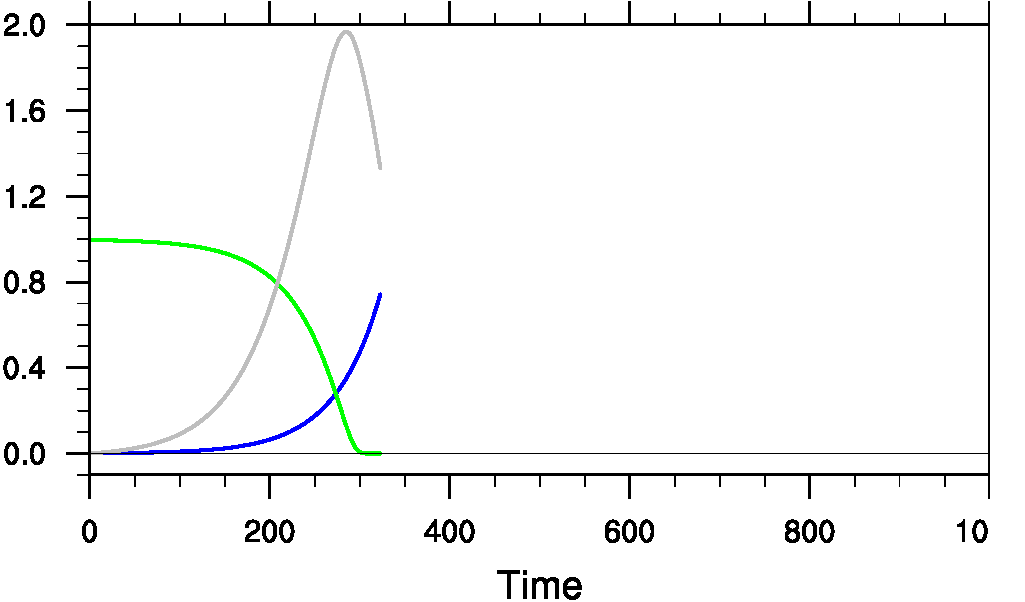
\includegraphics[width=0.7\linewidth]{../ncl/egalitarian-collapse-fe-01-lpos1-sp.pdf}
\captionof{figure}{Prolétaires (bleu, unité $\chi_M$), ressources naturelles (vert, unité $\lambda$) et richesses accumulées (gris, unité 10 $\lambda$), pour une société "egalitarian" dans la configuration "irreversible type-N collapse". La variable "ressources naturelles" devient négative au pas de temps 323, ce qui n'a plus de sens. \label{fig:egalitarian-collapse-fe-01-lpos1-sp}}
\end{center}

\section{Test de positivité}
On peut imposer en sortie du schéma numérique que toute valeur négative soit remise à zéro. Dans ce cas, la variable "ressources naturelles" est forcée à zéro au pas de temps 323 et le reste pour toute l'intégration puisque $\dot{y}$ est proportionnelle à $y$. La figure \ref{fig:egalitarian-collapse-fe-01-lpos2-sp} montre qu'on obtient alors un résultat semblable à la figure 3.d de l'article, c'est-à-dire un effondrement irréversible.

\begin{center}
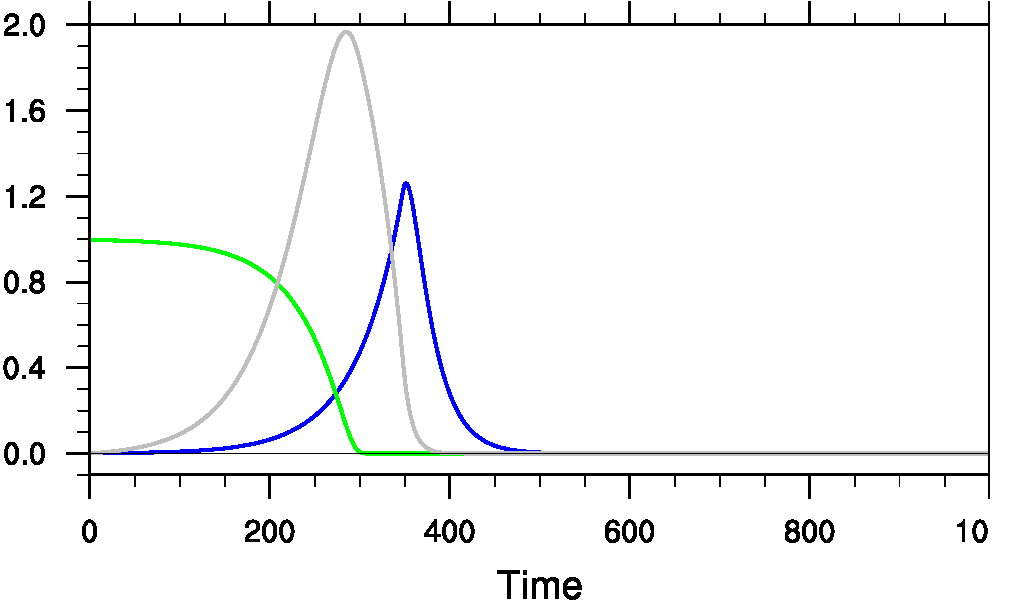
\includegraphics[width=0.7\linewidth]{../ncl/egalitarian-collapse-fe-01-lpos2-sp.pdf}
\captionof{figure}{Comme la figure \ref{fig:egalitarian-collapse-fe-01-lpos1-sp}, en ajoutant un test de positivité. \label{fig:egalitarian-collapse-fe-01-lpos2-sp}}
\end{center}

\section{Diminution du pas de temps}
Une autre stratégie pour améliorer la précision du schéma d'intégration Euler explicite est de diminuer le pas de temps. La figure \ref{fig:egalitarian-collapse-fe-02-lpos0-sp} montre qu'en divisant par deux le pas de temps (6 mois au lieu d'un an), le résultat obtenu est semblable à la figure 3.d de l'article, sans qu'un test de positivité ne soit nécessaire.

\begin{center}
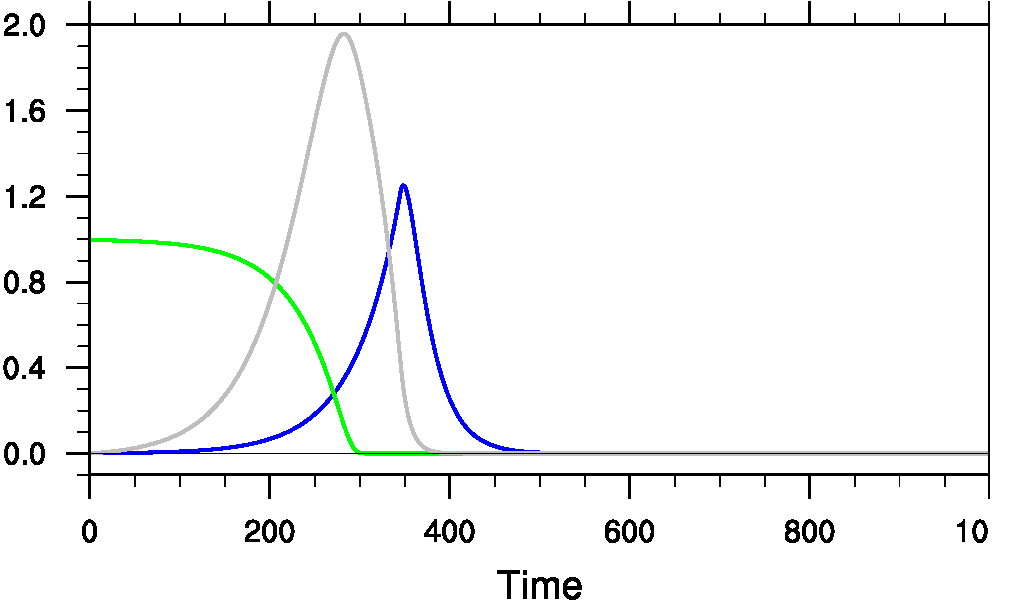
\includegraphics[width=0.7\linewidth]{../ncl/egalitarian-collapse-fe-02-lpos0-sp.pdf}
\captionof{figure}{Comme la figure \ref{fig:egalitarian-collapse-fe-01-lpos1-sp} avec un pas de temps de 6 mois au lieu d'un an. \label{fig:egalitarian-collapse-fe-02-lpos0-sp}}
\end{center}

\section{Schéma de Runge-Kutta}
Le schéma d'intégration Euler explicite est en général peu utilisé car, outre son instabilité, il est peu précis (schéma d'ordre 1). Un schéma très populaire pour les intégrations peu coûteuses comme le modèle HANDY est celui de Runge-Kutta d'ordre 4\footnote{\url{https://fr.wikipedia.org/wiki/M\%C3\%A9thodes\_de\_Runge-Kutta}}, stable et précis. \textbf{Deuxième surprise} : la figure \ref{fig:egalitarian-collapse-rk-01-lpos0-sp} montre qu'avec ce schéma, la configuration "irreversible type-N collapse" ne présente plus d'effondrement irréversible mais des effondrements réversibles périodiques, comme la configuration "reversible Type-N collapse" (figure 3.c de l'article).

\begin{center}
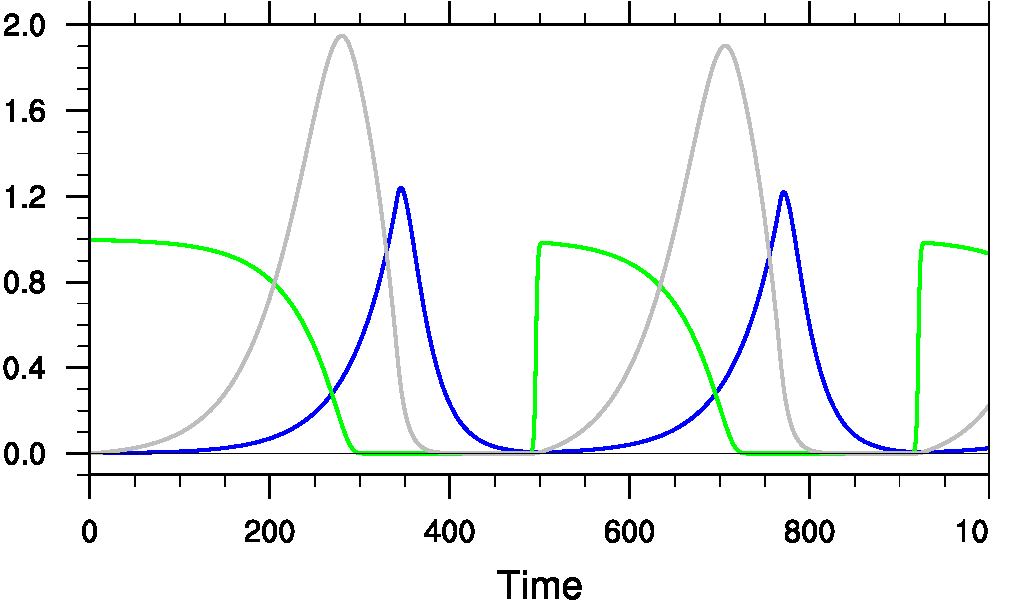
\includegraphics[width=0.7\linewidth]{../ncl/egalitarian-collapse-rk-01-lpos0-sp.pdf}
\captionof{figure}{Comme la figure \ref{fig:egalitarian-collapse-fe-01-lpos1-sp} avec un schéma de Runge-Kutta d'ordre 4. \label{fig:egalitarian-collapse-rk-01-lpos0-sp}}
\end{center}

\section{Traitement des petites valeurs}
Il semble que le modèle HANDY soit très sensible au schéma numérique choisi, en particulier lorsque les variables prennent des valeurs très faibles. Un traitement théorique et numérique propre serait d'ajouter des mécanismes de dépensation... ce dont les auteurs de l'article se targuent de ne pas avoir besoin. A titre d'exemple, on peut ajouter un mécanisme de dépensation simple sur les ressources naturelles : lorsque celles-ci sont trop faibles (par exemple inférieures à 10$^{-6} \ \lambda$), alors le terme de régénération des ressources naturelles ($\gamma y (\lambda-y)$) est désactivé, et ne peut plus être activé dans le reste de l'intégration. Concrètement, cela signifie que si l'environnement est trop dégradé, alors il ne parvient plus à se régénérer.\\
$  $\\
Dans le cas de la configuration "irreversible type-N collapse", cela permet d'obtenir un résultat semblable à la figure 3.d de l'article en utilisant le schéma numérique Runge-Kutta d'ordre 4 (figure \ref{fig:egalitarian-collapse-rk-01-lpos3-sp}). Par contre, cela modifie fortement les configurations "oscillatory approach to equilibrium" (figure 3.b dans l'article) et "reversible type-N collapse" (figure 3.c dans l'article) en les transformant en effondrements irréversibles (figures \ref{fig:egalitarian-oscillatory_landing-rk-01-lpos3-sp} et \ref{fig:egalitarian-cycles-rk-01-lpos3-sp} respectivement). Cette transformation est logique : un effondrement irréversible de type N est désormais inévitable dès que les ressources naturelles sont quasi-épuisées pendant l'intégration, ce qui est le cas pour les configurations "oscillatory approach to equilibrium" et "reversible type-N collapse" de l'article. On remarque aussi que pour ces deux configurations, les figures de l'articles présentent des augmentations violentes des ressources naturelles lorsque les populations s'effondrent. Les ressources naturelles passent alors en quelques années d'un état quasi-nul à leur valeur maximale. Ces variations brutales n'ont pas beaucoup de sens, et sont éliminées par le mécanisme de dépensation.

\begin{center}
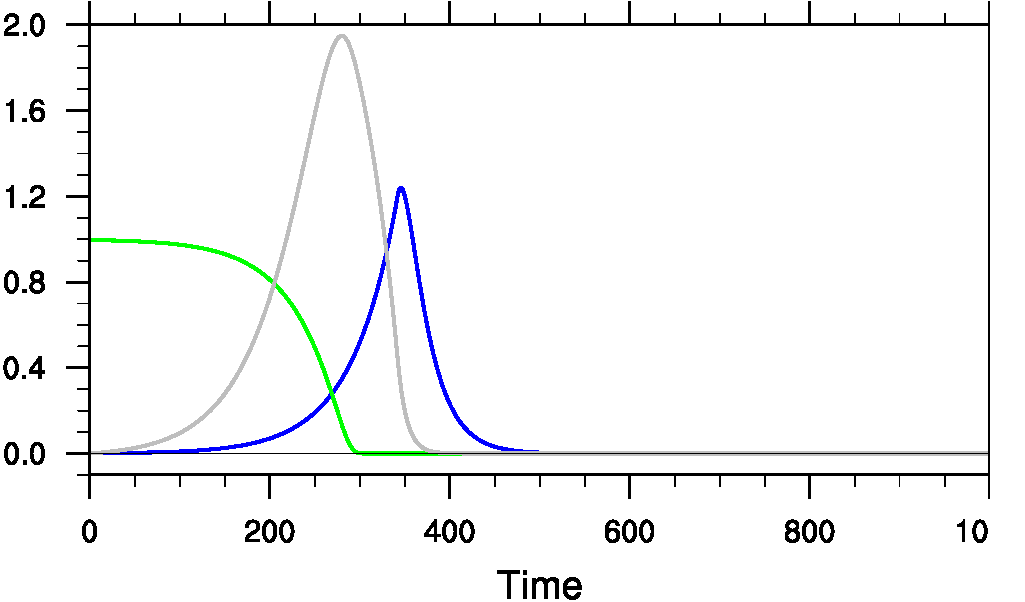
\includegraphics[width=0.7\linewidth]{../ncl/egalitarian-collapse-rk-01-lpos3-sp.pdf}
\captionof{figure}{Comme la figure \ref{fig:egalitarian-collapse-fe-01-lpos1-sp}, avec une dépensation des ressources naturelles. \label{fig:egalitarian-collapse-rk-01-lpos3-sp}}
\end{center}

\begin{center}
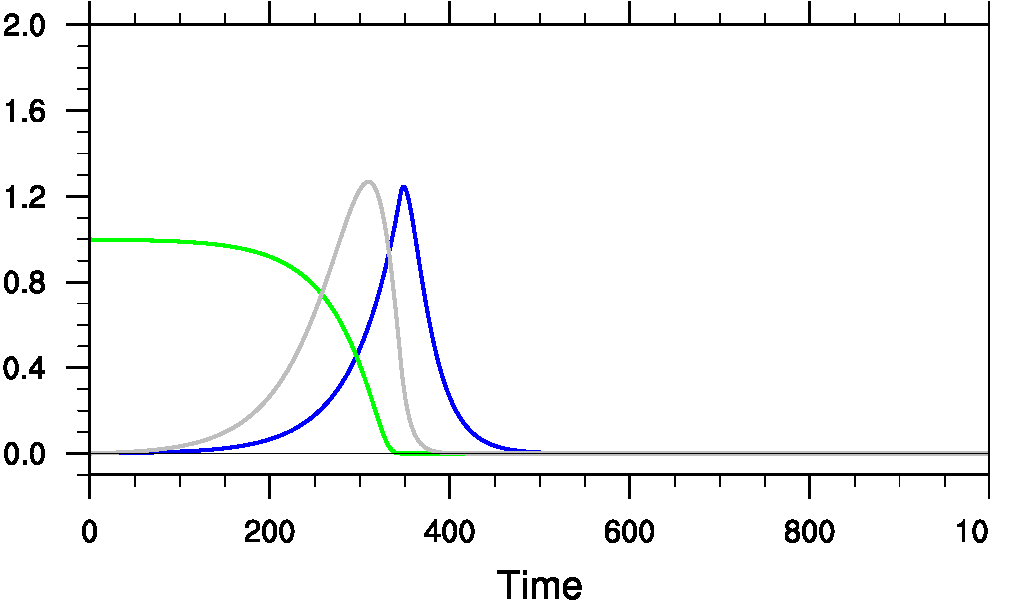
\includegraphics[width=0.7\linewidth]{../ncl/egalitarian-oscillatory_landing-rk-01-lpos3-sp.pdf}
\captionof{figure}{Comme la figure \ref{fig:egalitarian-collapse-fe-01-lpos1-sp} pour la configuration "oscillatory approach to equilibrium", avec une dépensation des ressources naturelles. \label{fig:egalitarian-oscillatory_landing-rk-01-lpos3-sp}}
\end{center}

\begin{center}
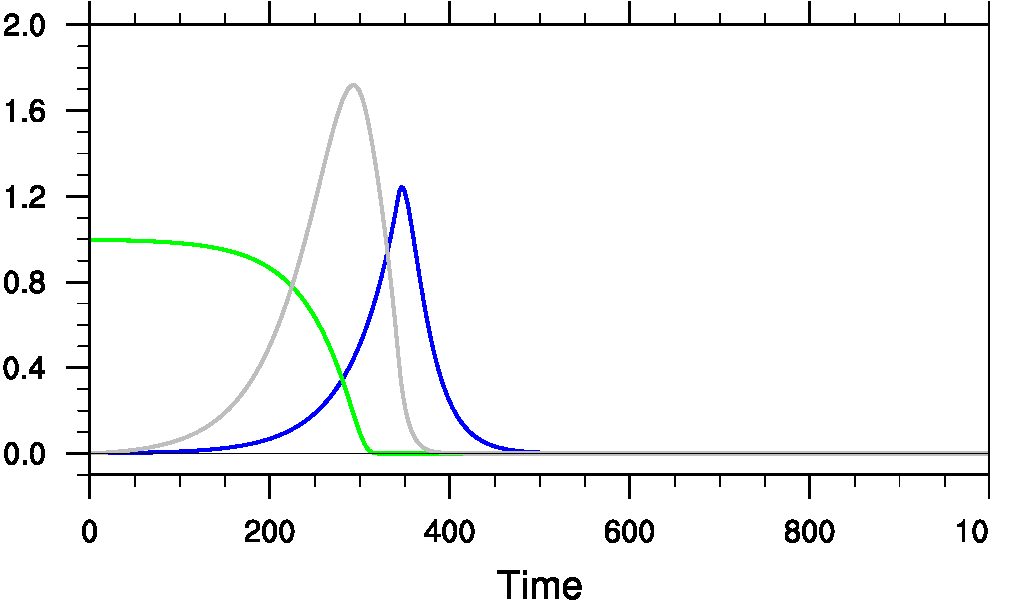
\includegraphics[width=0.7\linewidth]{../ncl/egalitarian-cycles-rk-01-lpos3-sp.pdf}
\captionof{figure}{Comme la figure \ref{fig:egalitarian-collapse-fe-01-lpos1-sp} pour la configuration "reversible type-N collapse", avec une dépensation des ressources naturelles. \label{fig:egalitarian-cycles-rk-01-lpos3-sp}}
\end{center}

\section{Conclusions}
Le modèle HANDY publié dans l'article \citet{motesharrei_2014} propose un jeu d'équation élégant pour modéliser de façon simple les interactions entre classes sociales, nature et richesse accumulée au sein d'un société, à partir d'hypothèses pertinentes. Il faut reconnaître la grande qualité de ce travail de mise en équation de phénomènes complexes.\\
$  $\\
Toutefois, notre étude montre que le choix du schéma numérique Euler explicite pour intégrer le modèle HANDY est désastreux pour la robustesses des conclusions de l'article. En effet, l'un des points forts de l'article - la présence "naturelle" d'effondrements irréversible en l'absence de mécanismes de dépensation - n'est qu'un résultat des erreurs numériques propres à ce schéma. Visiblement, les auteurs ont ajouté un test de positivité sans le mentionner. L'utilisation d'un schéma numérique plus précis (Runge-Kutta d'ordre 4) transforme ces effondrements irréversibles en effondrements réversibles. Sans pouvoir encore le prouver, je conjecture que le système d'équations de HANDY ne permet pas d'effondrements irréversibles, quelques soient ses paramètres, dès lors qu'un schéma numérique suffisamment précis et utilisé, avec un pas de temps suffisamment petit.
Cependant, si on ajoute à HANDY un mécanisme de dépensation simple sur les ressources naturelles, alors les situations de type "oscillatory approach to equilibrium" et "reversible type-N collapse" de l'article, peu crédibles, et mèneraient plutôt à des effondrements irréversibles.\\
$  $\\
Ces remarques n'auraient pas beaucoup d'importance si l'article \citet{motesharrei_2014} était un article de recherche peu connu, anecdotique. Ce n'est pas le cas. Cet article a été amplement commenté dans la presse (souvent de façon erronée), et il est maintenant au cœur des discours sur la collapsologie. Par exemple, ses conclusions ont été détaillées dans le livre "Comment tout peut s'effondrer. Petit manuel de collapsologie à l'usage des générations présentes" de Pablo Servigne et Raphaël Stevens (Seuil, 2015)\footnote{\url{http://www.seuil.com/ouvrage/comment-tout-peut-s-effondrer-pablo-servigne/9782021223316}}, et il figure même dans le manifeste du Comité Adrastia\footnote{\url{http://adrastia.org/qui-sommes-nous/manifeste}}. Un regard plus critique sur cet article, qui présente de graves défaillances, serait le bienvenu.

\bibliographystyle{mybib-en}
\bibliography{handy}

\end{document}
